% arara: makeindex

% Template for IEEE papers
%% bare_conf.tex
%% V1.4b
%% 2015/08/26
%% by Michael Shell
%% See:
%% http://www.michaelshell.org/
%% for current contact information.
%%
%% This is a skeleton file demonstrating the use of IEEEtran.cls
%% (requires IEEEtran.cls version 1.8b or later) with an IEEE
%% conference paper.
%%
%% Support sites:
%% http://www.michaelshell.org/tex/ieeetran/
%% http://www.ctan.org/pkg/ieeetran
%% and
%% http://www.ieee.org/

%%*************************************************************************
%% Legal Notice:
%% This code is offered as-is without any warranty either expressed or
%% implied; without even the implied warranty of MERCHANTABILITY or
%% FITNESS FOR A PARTICULAR PURPOSE!
%% User assumes all risk.
%% In no event shall the IEEE or any contributor to this code be liable for
%% any damages or losses, including, but not limited to, incidental,
%% consequential, or any other damages, resulting from the use or misuse
%% of any information contained here.
%%
%% All comments are the opinions of their respective authors and are not
%% necessarily endorsed by the IEEE.
%%
%% This work is distributed under the LaTeX Project Public License (LPPL)
%% ( http://www.latex-project.org/ ) version 1.3, and may be freely used,
%% distributed and modified. A copy of the LPPL, version 1.3, is included
%% in the base LaTeX documentation of all distributions of LaTeX released
%% 2003/12/01 or later.
%% Retain all contribution notices and credits.
%% ** Modified files should be clearly indicated as such, including  **
%% ** renaming them and changing author support contact information. **
%%*************************************************************************


% *** Authors should verify (and, if needed, correct) their LaTeX system  ***
% *** with the testflow diagnostic prior to trusting their LaTeX platform ***
% *** with production work. The IEEE's font choices and paper sizes can   ***
% *** trigger bugs that do not appear when using other class files.       ***                          ***
% The testflow support page is at:
% http://www.michaelshell.org/tex/testflow/

\documentclass{book}
\usepackage[quiet]{fontspec}
\usepackage[table,xcdraw,dvipsnames]{xcolor} % Used by spritegrid and others.
\usepackage[obeyspaces,spaces]{url}
\usepackage{longtable}
\usepackage{arydshln}
\usepackage{booktabs}
\usepackage{afterpage}
\usepackage{flushend}
\usepackage{titletoc}
\usepackage[toc]{appendix}
\usepackage{parskip}
\usepackage{graphicx,wrapfig}
\usepackage{float}
\usepackage{caption}
\usepackage{pdfpages}
\usepackage{tikzpagenodes}
\usepackage{imakeidx}
\usepackage[pagestyles,raggedright]{titlesec}
\usepackage[all]{nowidow}
\usepackage[bookmarks=true]{hyperref}
\usepackage{aeb-minitoc}
\usepackage{fix-cm}
\usepackage{textpos}
\usepackage{enumitem}
\usepackage{tcolorbox}
\tcbuselibrary{breakable,listings,skins,xparse}
%\usepackage{wrapfig}
\usepackage{needspace}
\usepackage{verbatim}
\usepackage{ean13isbn}
\usepackage{setspace}

% Use CHAPTER-PAGE page numbering to make it easier to modify chapters
% later, without messing up page number of the rest of the book.
\usepackage[auto]{chappg}

% Allow cross-references between the various books to the big The MEGA65 Book
\usepackage{xr}
\usepackage{varioref}
\usepackage{xparse}
\externaldocument[M65Book-]{mega65-book}
% And a \ref alternative that checks if it needs to be a cross-reference to the
% MEGA65 Book instead.
\makeatletter
\newcommand{\bookref}[1]{%
    \@ifundefined{r@#1}{%
      {\em the MEGA65 Book}, \nameref{M65Book-#1} (\autoref{M65Book-#1})}{\autoref{#1}}%
}
\newcommand{\bookvref}[1]{%
    \@ifundefined{r@#1}{%
      {\em the MEGA65 Book}, \nameref{M65Book-#1} (\autoref{M65Book-#1})}{Chapter/Appendix \vref{#1}}%
}
\makeatother

% For fixed-width columns in register maps
\usepackage{array}

% Makes tables with double-ruled lines look better
\usepackage{hhline}

% Makes better use of space for reference tables in appendix
\usepackage{multicol}

% Shaded tables with alternate rows colored for better legibility
% Best used with larger tables rather than small tables
\usepackage{colortbl}
\usepackage{adjustbox}
\usepackage[strict]{changepage}

% \makecell command for forcing line breaks in table cells
\usepackage{makecell}

\newcolumntype{L}[1]{>{\raggedright\let\newline\\\arraybackslash\hspace{0pt}}m{#1}}
\newcolumntype{C}[1]{>{\centering\let\newline\\\arraybackslash\hspace{0pt}}m{#1}}
\newcolumntype{R}[1]{>{\raggedleft\let\newline\\\arraybackslash\hspace{0pt}}m{#1}}

% For displaying Letter keys and the MEGA key
% This is a `keys' element for displaying a Mega65 keyboard key
% using a black filled label with rounded edges.
% In order to display a key as a title, use:
%
%     \megakey[title]{Run/Stop}
%
% For displaying a key as a part of the normal document flow, simply use:
%
%    \specialkey{SHIFT}
%
%
% If you get warnings on special characters, mathematical characters etc, use $, eg:
%
%    \megakey{$\leftarrow$}
%
% Other sizes are supported, as part of tcolorbox:
% http://mirror.aarnet.edu.au/pub/CTAN/macros/latex/contrib/tcolorbox/tcolorbox.pdf#subsubsection.4.7.5 however, only `title' and the default: `small' are proposed for use in this manual.
%
% The second macro available here is the megasymbolkey.
% This will display the MEGA symbol as white on a black key box. Simply use:
%
%		 \megasymbolkey
%
% Some MEGA65 keys contain two lines of text like "RUN/STOP"
% You can use the specialkey macro for this:
%
%    \specialkey{SHIFT LOCK}%

\usepackage{tcolorbox}

\newtcbox{\megakeyinner}[1][small]{colback=black, coltext=white, size=#1, fontupper=\bfseries, nobeforeafter,box align=bottom,baseline=3pt,text height=7pt}
\newcommand{\megakey}[2][small]{\megakeyinner[#1]{\uppercase{#2}}}

% Previous version of megasymbolkey
%\newtcbox{\megasymbolkeyinner}{colback=black, coltext=white, clip title=false. fontupper=\symbolfont, box align=bottom,baseline=3pt,text height=7pt}
%\newcommand{\megasymbolkey}{\megakeyinner{\megasymbol[white]}\ }

\newtcolorbox{megasymbolkeyinner}
{colback=black,coltext=white,size=small,fontupper=\small\bfseries,
width=0.65cm, height=0.55cm, box align=base,
nobeforeafter, halign=flush left, left=0mm,top=0.3mm,bottom=0mm,right=0mm
,boxsep=0.5mm,baseline=4pt, enlarge right by = 1mm
}
\newcommand{\megasymbolkey}{
\begin{megasymbolkeyinner}%
\megasymbol[white]%
\end{megasymbolkeyinner}%
}

\newtcolorbox{specialkeyinner}
{colback=black,coltext=white,size=small,fontupper=\tiny\bfseries,
width=0.80cm, height=0.55cm, box align=base,
nobeforeafter, halign=flush left, left=0mm,top=0.3mm,bottom=0mm,right=0mm
,boxsep=0.5mm,baseline=4pt
}
\newcommand{\specialkey}[1]{
\begin{specialkeyinner}%
#1%
\end{specialkeyinner}%
}

\newtcolorbox{widekeyinner}
{colback=black,coltext=white,size=small,fontupper=\tiny\bfseries,
width=0.9cm, height=0.55cm, box align=base,
nobeforeafter, halign=flush left, left=0mm,top=0.3mm,bottom=0mm,right=0mm
,boxsep=0.5mm,baseline=4pt
}
\newcommand{\widekey}[1]{
\begin{widekeyinner}%
#1%
\end{widekeyinner}%
}




% For displaying print versions petscii character symbols
% This is a collection of symbol macros element for displaying a printed version of the
% MEGA65 graphic characters, as opposed to the bitmap versions in the mega40/80.ttf fonts files.
% You can display characters using the graphicsymbol macro:
%
%    \graphicsymbol{\textcolor{red}{qQ} wWUcbdhjI \textcolor{blue}{JK}}
%
% Or you can, simply use the font itself:
%
%    \begin{symbolfont}%
%	   qQwWeErRtTyYuUiIoOpP\\
%		 aAsSdDfFgGhHjJkKlL\\
%		 zZxXcCvVbBnNmM%
%		 \end{symbolfont}%
%
%
% You can display the MEGA symbol using:
%
%    \megasymbol
%
% This will display the symbol in black. Other colours can be specified by passing them in, for example:
%
% 	 \megasymbol[black]
%		 \megasymbol[white]
%		 \megasymbol[orange]
%		 \megasymbol[blue]
%
% NOTE:
% For using the MEGA symbol in a key, see the \megasymbolkey macro in the keys.txt file.

\usepackage{tcolorbox}

\newcommand{\graphicsymbol}[1]{\begin{symbolfont}#1\end{symbolfont}}

\newcommand{\megasymbol}[1][black]{\begin{symbolfont}\textcolor{#1}{`}\end{symbolfont}}


% For Mega65 display of code, listings and screen activity
\input{elements/screenoutput}

% For MEGA65 screen shots with text flow
\input{elements/screenshots}

% For displaying sprite data in a grid
% This is an element for displaying a sprite in a grid, just like page 70 of the
% commodore manual. This version can be easily expanded. For now it will suffice.
% In order to display a hi-res mono sprite grid use:
%
%	\spritegrid{
%	\hline
%	\spritecells{---------ooooo----------}
%	\spritecells{-------ooooooooo--------}
%	\spritecells{------ooooooooooo-------}
%	\spritecells{------ooo--o---oo-------}
%	\spritecells{-----ooo-ooo-ooooo------}
%	\spritecells{-----ooo-ooo-ooooo------}
%	\spritecells{-----ooo---o---ooo------}
%	\spritecells{-----ooo-o-ooo-ooo------}
%	\spritecells{-----ooo-o-ooo-ooo------}
%	\spritecells{-----ooo---o--oooo------}
%	\spritecells{------ooooooooooo-------}
%	\spritecells{------ooooooooooo-------}
%	\spritecells{-------ooooooooo--------}
%	\spritecells{-------o-ooooo-o--------}
%	\spritecells{--------o-o-o-o---------}
%	\spritecells{--------o--o--o---------}
%	\spritecells{---------o-o-o----------}
%	\spritecells{---------o-o-o----------}
%	\spritecells{---------ooooo----------}
%	\spritecells{---------ooooo----------}
%	\spritecells{----------ooo-----------}
%	}
%
% For a multicolour sprite:
%
%	\spritegrid{
%	\hline
%	\spritecells{------------------------}
%	\spritecells{------------------------}
%	\spritecells{------------------------}
%	\spritecells{------------------------}
%	\spritecells{llllllllllllllllllllllll}
%	\spritecells{llllllllllllllllllllllll}
%	\spritecells{lllllleeeeeelleeeeeeeell}
%	\spritecells{lllloooooooollooooooooll}
%	\spritecells{llllooggggggllooggggggll}
%	\spritecells{lllloolllllllloollllllll}
%	\spritecells{llllooeeeellllooeeeellll}
%	\spritecells{lllloooooooollooooooooll}
%	\spritecells{llllooggggoollggggggooll}
%	\spritecells{lllloolllloollllllllooll}
%	\spritecells{llllooeeeeoolleeeeeeooll}
%	\spritecells{llllggooooggllooooooggll}
%	\spritecells{llllllggggllllggggggllll}
%	\spritecells{llllllllllllllllllllllll}
%	\spritecells{------------------------}
%	\spritecells{------------------------}
%	\spritecells{------------------------}
%	}

\usepackage{tabulary} %Removes spacing from tabulars
\usepackage{xstring} % for string substitution
\usepackage{xparse} % used for unpacking the sprite characters
% \renewcommand{\familydefault}{\sfdefault} % default sans font

%\usepackage{graphicx} % for resizing the tabular used by spritegrid
\usepackage{subcaption} % used for the left hand subtable of row numbers
\usepackage{multirow} % used for the ``Row'' column
\usepackage{rotating} % used by the rotating ``Row'' word

\newcommand{\spritebytecolumn}[1]{
   %\framebox[4mm]{#1}
   \makebox[4mm]{#1}
}

\setlength\tabcolsep{0.3mm} % the indivdual cell width and height


% Cell colour list. Can be expanded for other colours in the sprite grid
\def\blk{\cellcolor{black}}
\def\wht{\cellcolor{white}}
\def\grn{\cellcolor{ForestGreen}}
\def\lgrn{\cellcolor{YellowGreen}}
\def\gry{\cellcolor{Gray}}

\newcounter{lettercounter} % counter for detecting the last cell

% Collect the spritecell list and send it to \ProcessSpriteCell for turning into cells
\NewDocumentCommand{\spritecells}{%
>{\SplitList{}} m }{%
  \ProcessList{#1}{\ProcessSpriteCell}%
}

\NewDocumentCommand{\ProcessSpriteCell}{m}{%
  \stepcounter{lettercounter}%
    \IfStrEqCase{#1}{
	{o}{\blk}
	{-}{\wht}
	{g}{\grn}
	{l}{\lgrn}
	{e}{\gry}
   }%
   \IfStrEq{\thelettercounter}{24}{\setcounter{lettercounter}{0} \\ \hline}{&}%
}

% Start of the actual spritegrid definition
\newcommand{\spritegrid}[1]{
\begin{table}[h!]
\centering
\begin{subtable}{28mm}
\vspace{8mm}
\scalebox{0.76}{
\begin{center}
\begin{tabular}{p{25mm} p{4mm} c}
\multirow{21}{*}{ } &
\multirow{21}{*}{%
\begin{turn}{90}%
\bfseries\uppercase{Row}%
\end{turn}} &
 1\\
& & 2\\
& & 3\\
& & 4\\
& & 5\\
& & 6\\
& & 7\\
& & 8\\
& & 9\\
& & 10\\
& & 11\\
& & 12\\
& & 13\\
& & 14\\
& & 15\\
& & 16\\
& & 17\\
& & 18\\
& & 19\\
& & 20\\
& & 21
\end{tabular}
\end{center}
}
\end{subtable}%
\begin{subtable}{.8\textwidth}

\setlength{\arrayrulewidth}{1pt}
\scalebox{0.7}{
\begin{center}
\begin{tabular}{  *{3}{p{30mm} }  }
  \center\uppercase{Series\\1} &
  \center\uppercase{Series\\2} &
  \center\uppercase{Series\\3}
\end{tabular}
\end{center}
}

\scalebox{0.7}{
\begin{center}
\begin{tabular}{p{5.8mm} *{11}{C{7.3mm}}}
   128 & 32 & 8 & 2 & 128 & 32 & 8 & 2 & 128 & 32 & 8 & 2
\end{tabular}
\end{center}
}
\\[-1.5mm]
\scalebox{0.7}{
\begin{center}
\begin{tabular}{p{1.7mm} *{12}{C{7.3mm}}}
  & 64 & 16 & 4 & 1 & 64 & 16 & 4 & 1 & 64 & 16 & 4 & 1
\end{tabular}
\end{center}
}

\scalebox{0.7}{
\begin{center}
\begin{tabular}{ | *{24}{p{3mm} |}  }
#1
\end{tabular}
\end{center}
}

\scalebox{0.7}{
\begin{center}
\begin{tabular}{ *{24}{p{3.35mm}}  }
	\spritebytecolumn{1} & & & &
	\spritebytecolumn{5} & & & & &
	\spritebytecolumn{10} & & & & &
	\spritebytecolumn{15} & & & & &
	\spritebytecolumn{20} & & & &
	\spritebytecolumn{24} \\
	\multicolumn{24}{c}{\bfseries\uppercase{Column}}
\end{tabular}
\end{center}
}
\end{subtable}
\end{table}
}

% End of the actual spritegrid definition



% Don't number sections
\setcounter{secnumdepth}{0}

\renewcommand{\indexname}{INDEX}
\renewcommand{\appendixtocname}{APPENDICES}
\renewcommand{\appendixpagename}{APPENDICES}
\renewcommand{\appendixpage}{%
  \clearpage\thispagestyle{empty}
    \pagecolor{blue}
     \begin{center}
       {
         \large
         % Put a nice amount of vertical space before the title
         \vspace*{2cm}
               {\large\Huge\textcolor{white}{\bf{APPENDICES}}}\\
             \vspace{\fill}
       }
     \end{center}
     \newpage\pagecolor{white}\clearpage
}

\makeatletter\chardef\pdf@shellescape=\@ne\makeatother

\setcounter{tocdepth}{5}

% 1.0 cm is the distance from left of page to bullet point.
% 2.8 cm is a fudge-factor to make multi-line section names be correctly lined up.
% \@B{〈length〉} is the amount to indent prior to〈sec-num >
% \@F{〈fmt〉} is the formatting for the title heading
% \@P{〈fmt〉} is the formatting for the page number (〈pg-num〉).

\TOCLevels{chapter}{section}
\begin{minitocfmt}{\chapmtoc}
\declaretocfmt{section}{\@F{\color{white}\hspace{1.0cm}\textbullet\hspace{0.25cm}\Large\bfseries}\@B{2.8cm}\@P{\mtocgobble}}
\declaretocfmt{section*}{\@F{\color{white}\hspace{1.0cm}\textbullet\hspace{0.25cm}\Large\bfseries}\@B{2.8cm}\@P{\mtocgobble}}
\end{minitocfmt}

\input{fonts}

% Set margins for inner and outer pages in A5 book format
\ifdefined\printmanual
\usepackage[a5paper,nomarginpar,includemp,bottom=2cm,top=1cm,inner=1.8cm,outer=0.8cm, footskip = 1cm]{geometry}
\else
\usepackage[a5paper,nomarginpar,includemp,bottom=2cm,top=1cm,inner=1.0cm,outer=1.0cm, footskip = 1cm]{geometry}
\fi

% Some Computer Society conferences also require the compsoc mode option,
% but others use the standard conference format.
%
% If IEEEtran.cls has not been installed into the LaTeX system files,
% manually specify the path to it like:
% \documentclass[conference]{../sty/IEEEtran}

%% \input{setup}

% correct bad hyphenation here
\hyphenation{op-tical net-works semi-conduc-tor}

\makeindex[intoc]

\pagestyle{empty}

\begin{document}
\raggedbottom

% relax word wrapping with sloppy
\sloppy
% reduce overfull \hbox warnings
\hfuzz=5pt

% macro for changing the verbatim font
\makeatletter
\newcommand{\verbatimfont}[1]{\def\verbatim@font{#1}}%
\makeatother



%
% paper title
% Titles are generally capitalised except for words such as a, an, and, as,
% at, but, by, for, in, nor, of, on, or, the, to and up, which are usually
% not capitalised unless they are the first or last word of the title.
% Linebreaks \\ can be used within to get better formatting as desired.
% Do not put math or special symbols in the title.

\cleardoublepage

\pagenumbering{roman}


\newpagestyle{onlynumber}{\setfoot[][{\bf\small\thepage}][]
                                  {} {\bf\small\thepage} {}}
\pagestyle{onlynumber}
\pagecolor{white}

%% XXX - big numbers are not in bold, because latex gets confused
\newcommand*{\justifyheading}{\raggedleft}
\definecolor{headingblue}{rgb}{0.5,0.5,1}

% \titleformat{command}[shape]
%   {format}
%   {label}
%   {sep}
%   {before}
%   [after]

% ***************
% PART title page
% ***************

\titleclass{\part}{top}
\titleformat{\part}[display]
   {\thispagestyle{empty}\pagecolor{blue}\normalfont\huge\bfseries\justifyheading}
   {\textcolor{white}{\fontsize{50}{65}\selectfont\bf{PART}\quad{\fontsize{100}{130}\selectfont \bf{\serifed\thepart}}}}
   {20pt}
   {\Huge\textcolor{white}}
   [\newpage\pagecolor{white}\textcolor{black}]

% ******************
% CHAPTER title page
% ******************

\titleformat{\chapter}[display]
   {\thispagestyle{empty}\pagecolor{blue}\normalfont\huge\bfseries\justifyheading}
   {\textcolor{white}{\MakeUppercase{\chaptertitlename}\quad{\fontsize{100}{130}\selectfont \bf\thechapter}}}
   {20pt}
   {\Huge\textcolor{white}}
   [{\chapmtoc\insertminitoc}\newpage\pagecolor{white}\textcolor{black}\cleardoublepage]

% ******************
% SECTION title page
% ******************

\titleformat{\section}[display]
   {\raggedright}
   {\thesection}
   {20pt}
   {\huge\bf\color{headingblue}\uppercase}
   [\color{black}]

\pagenumbering{arabic}

          \chapter{Upgrading the MEGA65}

\section{How a MEGA65 Can Be Upgraded}
\label{cha:cores}

The MEGA65 platform consists of three major components:

\begin{enumerate}
  \item The {\bf MEGA65 core},\index{Core} a description of the chipset to run on the FPGA
  \item The {\bf ROM},\index{ROM} code that defines the Commodore-style operating system (KERNAL) and BASIC
  \item {\bf System software} for features such as the Freezer menu\index{Freezer menu}
\end{enumerate}

You can upgrade these components as new releases are published. You can also replace one or more of these components individually. In the case of the core and ROM, you can even have multiple versions installed simultaneously and switch between them. For example, instead of the latest MEGA65 ROM, you can switch to the original Commodore 65 prototype ROM. Or, you could switch to another core that causes your MEGA65 hardware to behave like a different computer entirely, such as a Commodore 64 or a ZX Spectrum.

The ROM and system software are files that reside on the SD card, and upgrading them is as simple as replacing the files. To upgrade the core, you use a process to install a core file into the MEGA65's core flash memory. This chapter describes this process.

\subsection{What is a Core?}
\index{Core!definition}

The MEGA65 hardware architecture is based on a versatile chip called a ``Field Programmable Gate Array,'' or FPGA.\index{Field Programmable Gate Array (FPGA)} This is a special kind of computer chip that can be programmed to impersonate other chips. They do this by configuring a giant array of logic gates to reproduce circuits. FPGAs are not an emulation, but an electronic re-creation of other chips. FPGA code is sometimes referred to as {\em firmware,} a term you may recognize from modern computers and other devices.

Your MEGA65 was programmed at the factory to re-create a chipset designed by the MEGA65 team, based on the original Commodore 65. You can re-program the MEGA65 FPGA to upgrade to new versions of the MEGA65 chipset, or to replace the chipset with that of an entirely different computer!

Each possible chipset is known as a {\em core}. The MEGA65 can store up to eight cores, and you can switch between these cores by accessing a menu when you switch on the computer. You can also use this menu to load a new core from a file on the SD card, a process known as {\em flashing}.

Members of the MEGA65 community have made several useful and fun alternate cores for the FPGA hardware. \href{https://github.com/MJoergen/C64MEGA65}{{\em C64 for MEGA65}} by MJoergen and sy2002 re-creates the original Commodore 64 computer with a high degree of accuracy, perfect for running Commodore 64 games, demos, and applications. Other cores re-create the ZX Spectrum, the Game Boy, and even the original Galaga arcade machine hardware. The MEGA65 team believes that the FPGA is powerful enough to re-create nearly all 8-bit home computers, and likely some 16-bit computers and consoles such as the Commodore Amiga. The MEGA65 hardware design, board layout, FPGA core, and other information are all available for free under various open-source licenses, so anyone is free to create other cores for the MEGA65 hardware.

\section{Determining the Versions of Things}
\label{sec:versions}

All components of the MEGA65 platform have a version identifier. The MEGA65 can display the version identifiers for all of its components using the MEGA65 Information utility.\index{MEGA65 Information Utility}

To open the MEGA65 Information utility:

\begin{enumerate}
  \item Switch on the MEGA65, and allow it to boot to BASIC.
  \item Open the Freezer:\index{Freezer menu} press and hold \widekey{RESTORE} for one second then release it.
  \item Press \specialkey{HELP}. The MEGA65 Information utility will open.
\end{enumerate}

\begin{center}
  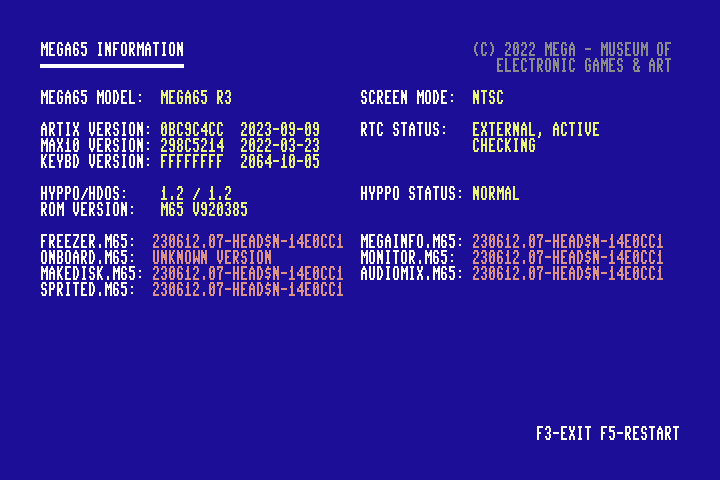
\includegraphics[width=0.7\linewidth]{images/megainfo.png}
\end{center}

Take note of these version identifiers:
\nopagebreak
\begin{center}
\setlength{\tabcolsep}{1mm}
\begin{tabularx}{\textwidth}{|X|p{7cm}|}
  \hline
  {\bf Label and Example} & {\bf Description} \\
  \hline
  MEGA65 Model\newline {\tt MEGA65 R5} & The revision of the hardware. You need to know this when downloading new core files. \\
  \hline
  Artix Version\index{Core!Version}\newline {\tt 93D55F08 2022-10-12} & The currently running MEGA65 core. This is a string of eight letters and numbers, and also a build date. \\
  \hline
  ROM Version\index{ROM!Version}\newline {\tt M65 V920377} & The currently running ROM. For MEGA65 ROMs, this is a sequential number, with larger numbers representing newer releases. \\
  \hline
  System files (.M65)\newline {\tt 221012.18-MASTER-5BBFDA9} & Each of the system software files has its own version identifier. Typically, you do not need to know these: you will upgrade these along with each core. The identifier is similar to the core version, but does not always match the currently running core. \\
  \hline
\end{tabularx}
\end{center}

Press \specialkey{F3} to exit to the Freezer, then \specialkey{F3} again to exit to BASIC.

Each core has a separate version for each hardware revision. As of the year 2023, the production models of the MEGA65 have used two different main board revisions, known as ``R3'' (more specifically ``R3A'') and ``R5.''\footnote{The MEGA65 ``DevKit'' model sold in the year 2020 is revision ``R3.'' It is also possible to run the MEGA65 core on certain FPGA development boards, with a separate version of the core file for each.}\index{Hardware revisions}

The MEGA65 core is available for all hardware revisions. If you are installing an alternate core and it is not available for your hardware revision, contact the author of the core.

\section{Obtaining the Latest Files}

You can download the latest MEGA65 core, ROM, and system software from the MEGA65 Filehost website.\index{Filehost website} Due to distribution restrictions for the Commodore 65 ROM code, some files require a Filehost account registered to a MEGA65 owner to access. All owners of the MEGA65 have a license to all versions of this ROM code.\footnote{There is a procedure for non-owners to get the latest MEGA65 ROM, such as to use with the \href{https://github.lgb.hu/xemu/}{Xemu MEGA65 emulator}. This involves downloading \href{https://www.c64forever.com/}{C64 Forever Free Express Edition} from Cloanto, extracting the original Commodore 65 prototype ROM file, then using a tool to apply a patch that you can download from Filehost. The full process is described in the following article: \url{https://files.mega65.org?ar=145591dd-deb6-4bd0-aa89-8e39cd021470}}

Visit the following URL in your web browser:

\url{https://files.mega65.org}

\begin{center}
  \fbox{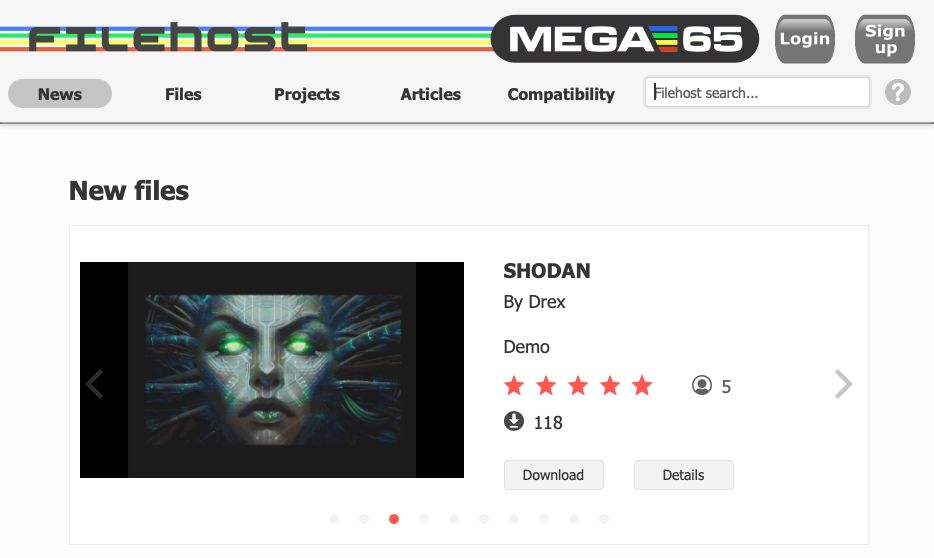
\includegraphics[width=0.7\linewidth]{images/filehost_notsignedin.png}}
\end{center}

To register a Filehost account with your owner code:

\begin{enumerate}
  \item Visit \href{https://files.mega65.org}{the Filehost website}. Click ``Sign Up.'' Follow the prompts to create an account.
  \item Locate your owner code.\index{Owner Code} This is a code printed on a piece of paper that was included with your MEGA65 (possibly inserted into this manual). It looks something like this: {\tt 123-ABC-456}
  \item Click the user icon in the upper-right corner of the Filehost screen. In the pop-up menu, select ``Redeem Code.'' Enter your owner code as prompted.
\end{enumerate}

\begin{center}
  \fbox{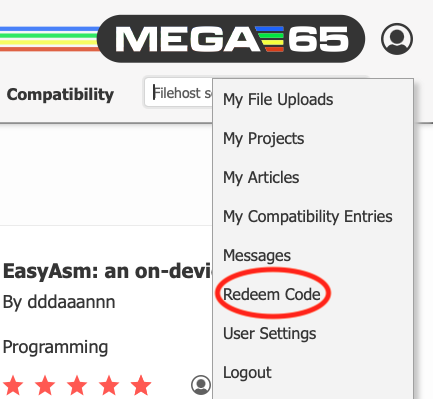
\includegraphics[width=0.4\linewidth]{images/filehost_redeemmenu.png}}
\end{center}

To download the latest release package:

\begin{enumerate}
  \item Click the ``Files'' tab of the Filehost website.
  \item In the search box on the left-hand side, type: ``release'' The list will update to show only files with that word in the title.
  \item Locate the entry named, ``MEGA65 Core Release Package (mega65r5) incl. ROM,'' where ``mega65r5'' matches your hardware revision. (To confirm your hardware revision, open the Freezer menu, then press \specialkey{Help}.)
  \item Click the entry. Confirm that this release package is for your hardware revision, then click ``Download'' to download the file.
\end{enumerate}

If you don't see an entry that says ``incl. ROM,'' check that you are signed in and that you have redeemed a valid owner code. Note that there is an entry for the Release Package that does not include the ROM that is visible to everyone. To ensure you are using a compatible set of files, get the package that says ``incl. ROM.''

\begin{center}
  \fbox{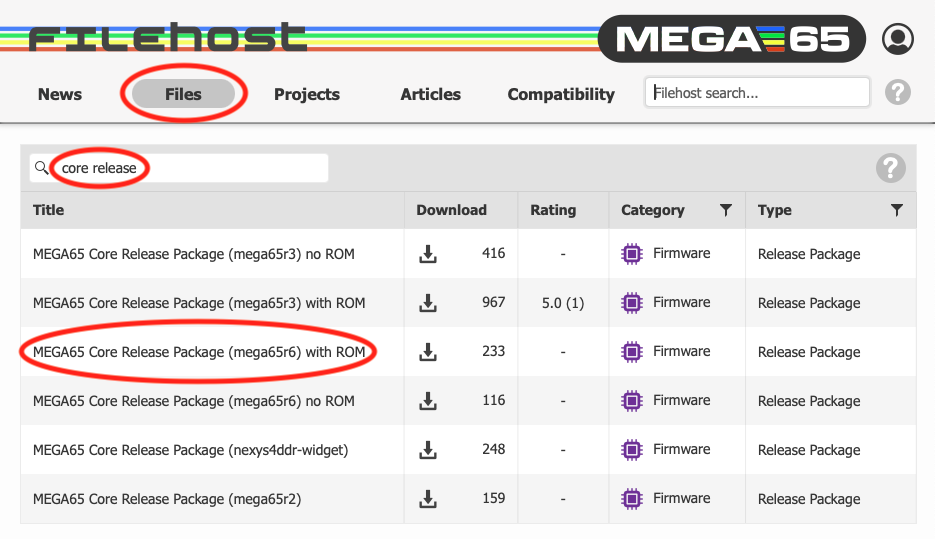
\includegraphics[width=0.7\linewidth]{images/filehost_release.png}}
\end{center}

Extract the downloaded {\tt .7z} archive. You should see a file whose name ends in {\tt .cor}, and a folder of {\tt sdcard-files} that includes one named {\tt MEGA65.ROM}.

\section{The Core Selection Menu}
\index{Core!Core Selection Menu}

The MEGA65 decides which core to load into the FPGA when it starts up. You can interrupt this process to select which core to load.\footnote{Technically, the MEGA65 starts the core in slot 0 to power the core selection menu. After you have made a selection or it chooses a default, it loads the selected core into the FPGA and continues the boot process.}

To open the core selection menu, switch off the computer, then hold the \specialkey{NO\\SCROLL} key and switch on the computer. The core selection menu appears, with the eight core slots numbered 0 through 7.

\begin{center}
  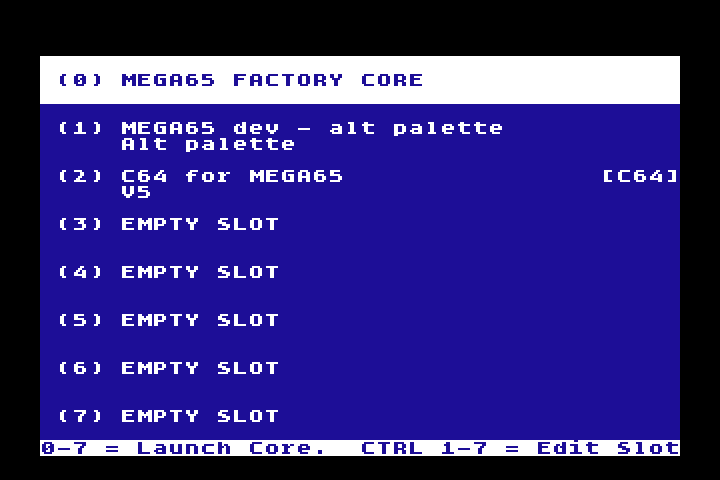
\includegraphics[width=0.7\linewidth]{images/ss-flashmenu.png}
\end{center}

You can select a core to boot using the cursor keys and \specialkey{RETURN}, or you can simply press the number key that corresponds to the slot. The boot process continues with the new core. The MEGA65 will keep running the new core until you physically power it off. (Pressing the reset button will not reset which core is being run.)

When you switch on the computer without opening the core selection menu, the MEGA65 looks for a core in slot 1. If there is a valid core in that slot, it uses it. Otherwise it tries slot 0.\footnote{You can change the default core slot from 1 to 2 by moving DIP switch \#4 to the ``on'' position. DIP switches are located inside the case, on the main board. For a diagram of the DIP switch locations, see \vref{cha:transferring-files}.}

Your computer comes with the MEGA65 core in slot 0 installed at the factory. It is recommended that you do not upgrade the factory-installed core under most circumstances. Instead, install new versions of the MEGA65 core in slot 1.

\section{Upgrading the MEGA65 Core, ROM, and System Files}
\index{Core!Upgrading}\index{ROM!Upgrading}

You can upgrade a core or install a new core from the core selection menu. This process reads the {\tt .cor} file from the SD card.

To upgrade the MEGA65 core, ROM, and system files:

\begin{enumerate}
  \item Remove the SD card (or microSD card) from the MEGA65, and connect it to your PC using an SD card reader.\footnote{As an alternative to moving the SD card to your PC, you can transfer files using an Ethernet connection. See chapter \vref{cha:transferring-files}.}
  \item Copy the {\tt .cor} file that you extracted from the {\tt .7z} archive to the SD card.
  \item On your PC, open the {\tt sdcard-files} folder from the {\tt .7z} archive, then copy those files to the SD card, replacing the existing files. Put them in the root of the SD card's file system, not a sub-folder.
  \item Eject the SD card from your PC's operating system, then move it back to the MEGA65.
  \item Open the core selection menu: Switch off the MEGA65, then hold \specialkey{NO\\SCROLL} while switching it back on.
  \item Hold \specialkey{CTRL} then press the number of the slot you want to upgrade. Follow the prompts. This process asks for a key press several times, and takes several minutes.
\end{enumerate}

When you start the update process, it prompts you to select the {\tt .cor} file on a screen that looks similar to this:

\begin{center}
  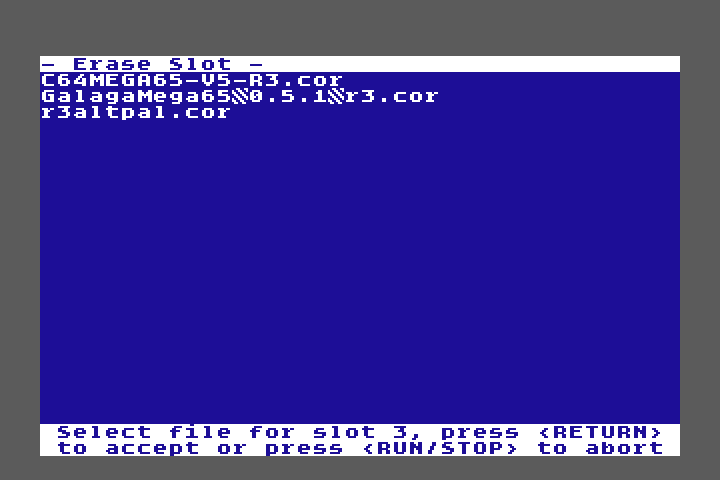
\includegraphics[width=0.7\linewidth]{images/ss-flashmenu-selectcore.png}
\end{center}

The process begins by checking that the core file matches your hardware revision. Press any key to continue.

\begin{center}
  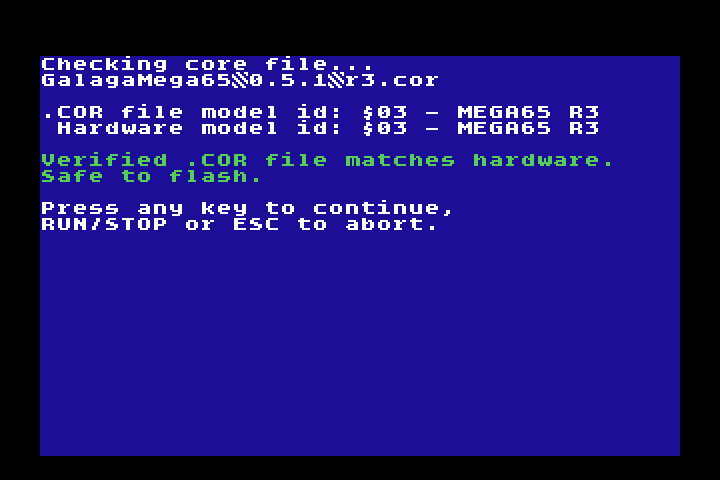
\includegraphics[width=0.7\linewidth]{images/ss-flashmenu-1-checking.png}
\end{center}

It then copies the file from the SD card to RAM, performing another check that the core file is complete.

\begin{center}
  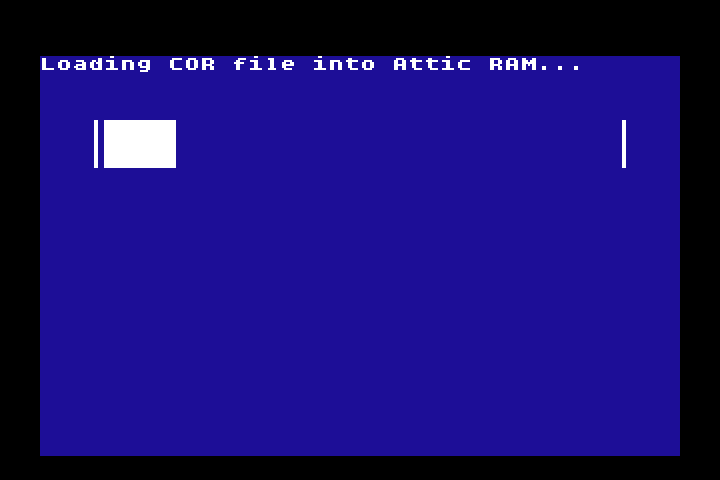
\includegraphics[width=0.7\linewidth]{images/ss-flashmenu-2-loading.png}
\end{center}

It presents the result of this check before proceeding. If the check is valid, you will see a message similar to the following. Press any key to continue.

\begin{center}
  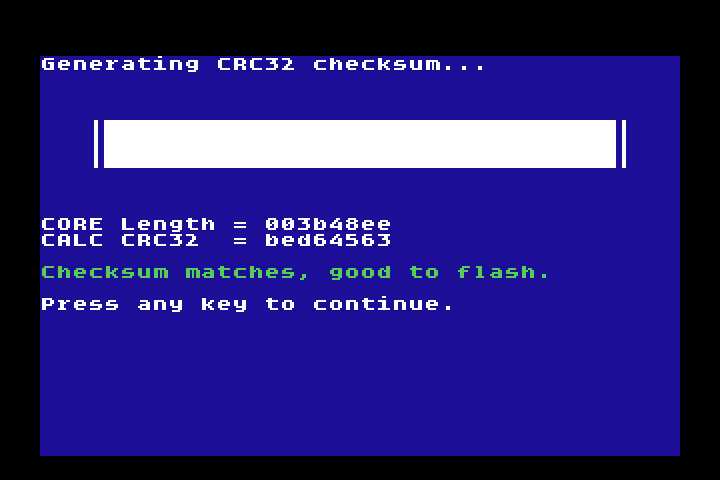
\includegraphics[width=0.7\linewidth]{images/ss-flashmenu-3-checksum-ok.png}
\end{center}

If the check is invalid, you will see the message, ``CHECKSUM MISMATCH.'' If you were not expecting this message, abort the process and confirm that you are using the correct file.\footnote{There are rare cases where a core may be valid but not have a correct checksum, such as if you are installing older versions of the core.}

Once you tell it to proceed, the MEGA65 begins programming the core data into flash memory. The border twinkles in coloured patterns during this process.

\underline{Note}: Do {\em not} switch off your computer or disconnect power until after this step is complete.

\begin{center}
  \fbox{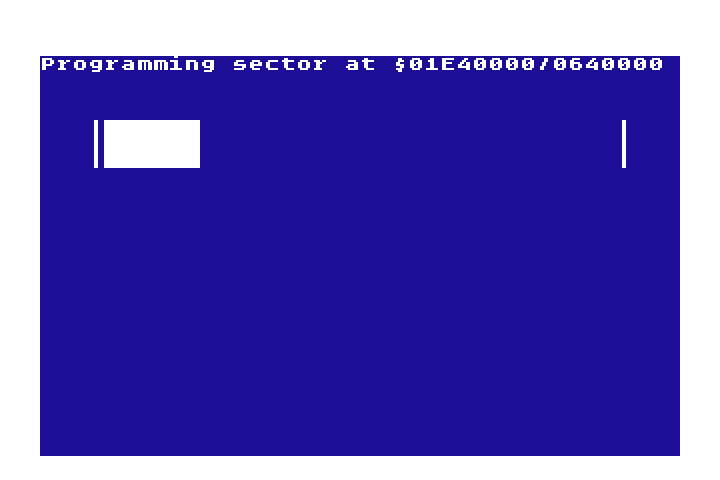
\includegraphics[width=0.7\linewidth]{images/ss-flashmenu-4-programming.png}}
\end{center}

When the process is complete, you will see a screen similar to the following.

\begin{center}
  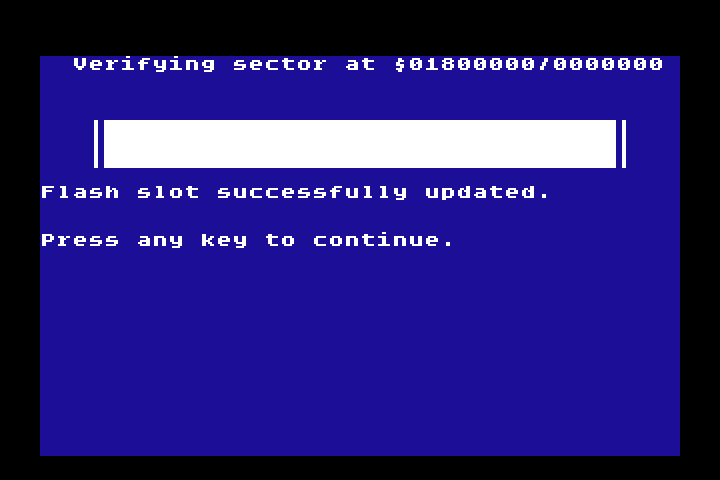
\includegraphics[width=0.7\linewidth]{images/ss-flashmenu-done.png}
\end{center}

It is now safe to switch off your computer. Press any key to return to the core selection menu, or switch the computer off then on again to start the default core.


\section{Installing Alternate Cores}

Installing an alternate core, such as the C64 core,\index{Core!C64 core} uses the same steps for flashing the core to a slot.

It is recommended to use slots 2 through 7 for alternate cores, and reserve slot 1 for the latest MEGA65 core. Of course, there is nothing stopping you from installing an alternate core in slot 1, so that the MEGA65 behaves as a different type of computer when you switch it on. You can always choose the MEGA65 core from the core selection menu.


% TODO: Document how to configure the boot core for cartridge types


\section{Upgrading the Factory Core in Slot 0}
\index{Core!Upgrading Slot 0}

It is possible to upgrade the factory-installed MEGA65 core in slot 0. You only need to do this in rare cases, such as if a newer version of the MEGA65 core includes changes or bug fixes for the start-up process. The process is elaborate, delicate, and could result in a MEGA65 that fails to start if something goes wrong. It is {\em strongly} recommended that you do not upgrade slot 0 unless the announcement for the release suggests that you do so. Most MEGA65 core upgrades are fully functional in slot 1, without needing to upgrade slot 0.

{\em Please read these instructions carefully before starting the procedure.}

\begin{enumerate}
  \item Prepare to use the {\em internal SD card only}. This may involve opening the case to make the SD card easier to access. Do {\em not} use the external microSD card slot for updating core slot 0.
  \item Using your PC, rename the core file that you wish to install to this exact filename: {\tt UPGRADE0.COR} (That's the word {\tt UPGRADE}, the number zero, and {\tt .COR}, using uppercase letters.)
  \item Install the latest MEGA65 core in slot 1, using the procedure described earlier. The core must be in the default non-zero slot to recover from any problems when updating slot 0. Boot this core to test that it works.
  \item Open the core selection menu. Press \megasymbolkey and the comma key to start the flash procedure for slot 0. (You will not be prompted for a filename.)
\end{enumerate}

\ifdefined\printmanual
\else
\underline{Note}: If you have a revision R3A MEGA65, have not previously upgraded slot 0, and \megasymbolkey and \megakey{,} does not start the procedure, you have an older slot 0 core that does not have this feature. You can work around this by restarting the core selection menu with slot 1. From the core selection menu, prepare to hold down \specialkey{NO\\SCROLL}, press the \megakey{1} key to boot into the core then immediately press and hold \specialkey{NO\\SCROLL}. The core selection menu re-opens using slot 1. Press \megasymbolkey and the comma key to complete the slot 0 upgrade.
\fi

If something goes wrong during the slot 0 flashing process, your MEGA65 may not start correctly. Before doing anything else, switch on your MEGA65, and wait a minute or so. It should notice that there is no valid core in slot 0, then proceed to start the core in slot 1. You can hold \specialkey{NO\\SCROLL} during this to open slot 1's core selection menu and restart the flashing process.

If the MEGA65 cannot boot any core after several minutes, it may be stuck. You may be able to recover using a device known as a ``JTAG interface'' that connects your PC to the MEGA65 main board. This allows you to inject a bitstream directly into the FPGA. The part is inexpensive but not always available. Contact the MEGA65 team on the Discord (\url{https://mega65.org/chat}) for assistance.


\section{Installing Alternate ROMs}

You can keep more than one version of the MEGA65 ROM on the SD card. When booting the MEGA65 core, you can select one of these ROMs by holding down a number key during boot.

To install alternate ROMs, copy them to the root of the SD card with a filename such as {\tt MEGA65x.ROM}, where {\tt x} is a number between 1 and 7. To boot the alternate ROM, hold the corresponding number key down while the MEGA65 core starts. If you do not hold down a number, it boots to {\tt MEGA65.ROM} by default.

There are several reasons you might want to keep alternate ROMs on your SD card:

\begin{itemize}
  \item You are helping to test a new beta release of the ROM, and do not wish to make the beta version your default ROM.
  \item You want to try the MEGA65 OpenROM, a project to create an all-new ROM released under an Open Source license without any original Commodore material.
  \item You want to try the original Commodore 65 prototype ROM. The MEGA65 core maintains backwards compatibility with the C65 ROM that was in progress by Commodore before they cancelled the project. It is buggy and incomplete, but is still an interesting historical artifact.
\end{itemize}

Several alternate ROMs came with your MEGA65 SD card, installed at the factory. Try rebooting your computer while holding down a number key to see what happens!


\section{Understanding The Core Booting Process}
\nopagebreak
This section summarises how the MEGA65 selects which core to start with when it is switched on. The process is shown in the following figure:
\nopagebreak
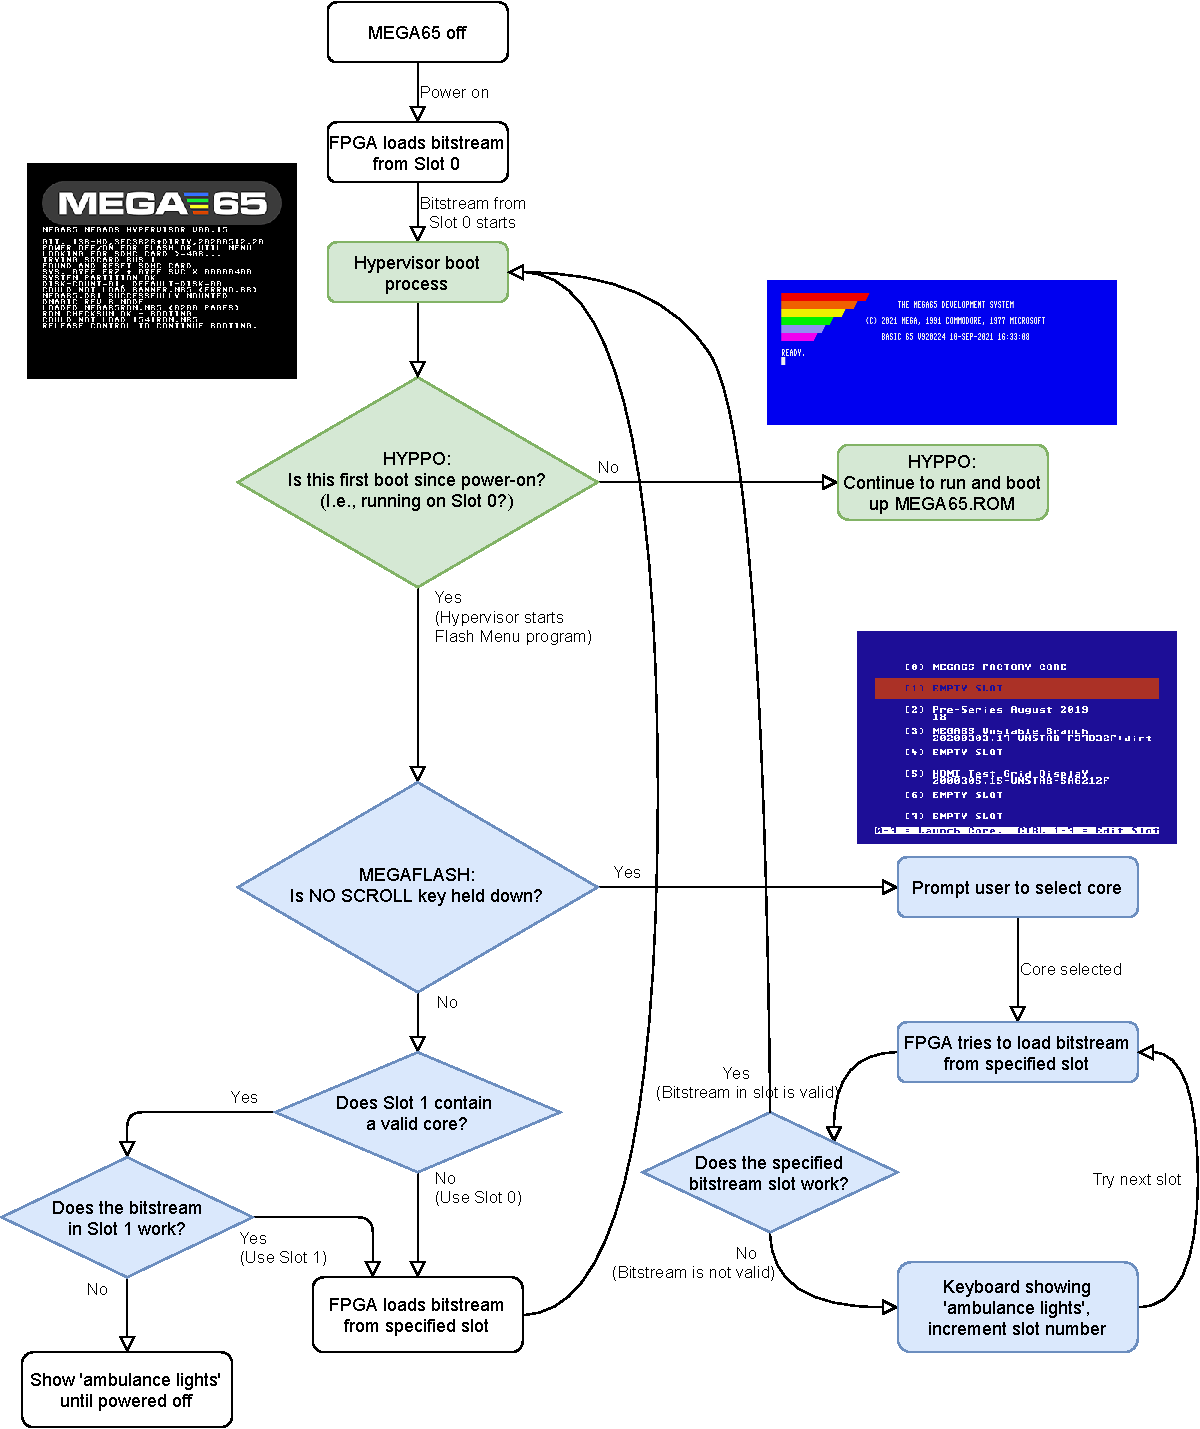
\includegraphics[width=\linewidth]{images/illustrations/flashmenu-flowchart.pdf}

The booting process is governed by two facilities:
\begin{itemize}
  \item The Hypervisor (also known as HYPPO), which operates at a level above the KERNAL. One of its responsibilities is to manage aspects of the boot process. For more details on the Hypervisor, refer to
\ifdefined\printmanual
the {\bf MEGA65 Book}.
\else
 \bookvref{sec:hypervisor-mode}.
\fi
    In the diagram, activities performed by the Hypervisor have been highlighted in green.
  \item The Core Selection Menu program (also known as ``MegaFlash''), which provides a list of available core slots to choose from. In the diagram, activities performed by MegaFlash have been highlighted in blue.
\end{itemize}

When the MEGA65 is switched on, it does the following:
\begin{itemize}
\item Loads the bitstream stored in slot 0 of flash memory. If that is the MEGA65 Factory Core, the MEGA65
  HYPPO Hypervisor starts.
\item If it is the first boot since power-on (which implies that you are running from slot 0), HYPPO starts the Flash Menu program (aka MegaFlash) -- but note that the Flash Menu in
      this mode may not show anything on the screen to indicate that it is running!
\item The Flash Menu then checks if \specialkey{NO\\SCROLL} is being held down.
\item If it is, the Flash Menu program shows its display, allowing you to select or re-flash a core.
\item If \specialkey{NO\\SCROLL} is {\em not} being held down, the Flash Menu program checks if Flash Slot 1 contains a valid
      core.
\item If it does, then the Flash Menu program attempts to load that core.
\item If it succeeds, then the system reconfigures itself for that core, after which the behaviour of the system is
      according to that core.
\item If it fails, the keyboard will go into ``ambulance mode'', showing flashing blue lights to indicate that some
      first-aid is required. Note that in ambulance mode the reset button has no effect: You must switch the
      MEGA65 off and on again.
\end{itemize}

If you have selected a different core in the Core Selection Menu, the process is similar, except that the ambulance lights will appear for only a limited time, as the FPGA will automatically search through the flash memory until it finds a valid core. If it gets to the end of the flash memory, it will start the MEGA65 Factory Core from slot 0 again.


\part{APPENDICES}

\begin{appendices}


\end{appendices}



\include{common-footer}
